\documentclass[../main.tex]{subfiles}

\begin{document}

\section{Materials and Methods}

\subsection{Microscopy}

A substantial amount of work for this project has been on determining the optimal microscopy technique for the live imaging of protein clustering.

\subsubsection{Main Microscopy Setup}

The microscope used after trialling was as follows:

\begin{itemize}
\item{Nikon Eclipse Ti-E Inverted Microscope}
\item{40X 0.6NA long working distance plan objective}
\item{100X 1.49NA TIRF oil plan apo objective}
\item{Andor iXon 897 Ultra 512x512 pixel \SI{16}{\micro\meter} EM CCD camera}
\end{itemize}

An OptoSplit II system from Cairn was employed to visualise Homo- and Hetero- FRET measurements simultaneously. This unit is placed in the lightpath between the microscope and the camera. Within it, a dichroic and pair of filters project the same half of the image onto each half of the camera sensor in different wavelengths or polarisation orientations. It is also possible to block one light path and allow the other to fully occupy the camera sensor by means of adjusting mirrors and shutters.

Inside the OptoSplit II is a dichroic and two filters (one in the case of anisotropy). Whilst there is already good wavelength filtering by the excitation and emission dichroics, the filters are required to clean up the signal and remove any longer wavelengths.

\paragraph{Excitation} was achieved with the following LED lighting system
\begin{center}
\begin{tabular}{l|c|c|l}
\textbf{Description}	&	\textbf{LED wavelength}	&	\textbf{Filter}	&	\textbf{Location} \\\hline
mCherry	&	White	&	560/40x	&	Back	\\
YFP		&	505		&	500/20x	&	Back\\
GFP		&	470		&	470/40x	&	Back\\
Blue		&	White	&	440/10x	&	Back\\
Bright Field		&	White	&	590	&	Top
\end{tabular}
\end{center}

Only one blue (GFP or Blue) LED could be used at any one time. Lights from the back were combined sequentially with a \SI{515}{\nano\meter} and \SI{495}{\nano\meter} dichroic.

The white light for bright field has a red (\SI{590}{\nano\meter}) filter placed in front of it as the white LED requires a phosphorescent element to achieve the right spread of wavelengths. This phosphorescent element can be excited by fluorescence excitation, causing a high level of light to be reflected back through the lens and into the camera. The red filter blocks this transmission and allows for rapid switching between bright field and fluorescent excitation without having to block the light path.

For anisotropy measurements, a rotating linear polariser could be inserted in front of the YFP LED.

The entire microscope is mounted on a ThorLabs PerformancePlus Series II breadboard fitted to a ThorLabs Active Isolation frame. This was felt necessary due to the presence of noisy machinery in adjacent rooms and high foot traffic.

\paragraph{Emission} was controlled with the following set of filters.
\begin{center}
\begin{tabular}{l|c|c|c|c|c}
&	\multicolumn{2}{c|}{Filter Wheel}	&	\multicolumn{3}{c}{OptoSplit II}	\\
\textbf{Description}	&	\textbf{Dichroic}	&	\textbf{Filter}		& \textbf{Dichroic}	&	\textbf{Filter 1}	&	\textbf{Filter 2}	\\\hline
YFP		&	515		&	535/30	&	-	&	-	&	-	\\
mCherry	&	585		&	630/75	&	-	&	-	&	-	\\
GFP		&	495		&	525/50	&	-	&	-	&	-	\\
YFP/mCherry Fret	&	515	&	-	&	565	&	545/40	&	630/75	\\
YFP Anisotropy	&	515	&	535/30	&	Polarising	&	Polarising	&	-	\\
Bright field		&	-	&	-	&	-	&	-	&	-	
\end{tabular}
\end{center}


\subsubsection{Fluorescent Proteins}

With kind support from other sources (see section~\ref{sec:plaspri:plas}) we built up a library of many fluorescent protein-chemotaxis protein fusions. However, it was still necessary to exchange many of these. Many fluorescent proteins\myfootnote{CFP, YFP, BFP and further derivatives} are all derivatives of GFP through only a few amino acid substitutions\cite{tsien98}. In most modernly used GFP derivatives, these all lie between amino acid 64 and amino acid 206, inclusive. Therefore, through careful design of PCR primers Gibson assembly can be used to exchange one GFP derivative for another with the same set of primers (see section~\ref{sec:plaspri:pri}).

Primarily EYFP was used for the proteins being imaged. However, a monomeric form was required for anisotropy\cite{vaknin07}, requiring the mutation A206K. Another EYFP varaent, known as Venus, was described as being a better FRET receiver\cite{nagai02} as well as a generally improved fluorophore, and therefore ideal for our anisotropy experiments. However, only the monomeric EYFP variant was available to us, and we have not yet had time to perform the five amino acid substitutions required for Venus.

\subsubsection{Inducer Calibration}

Most fusion proteins were available, or could easily be made available, in both the pBAD33 or pTRC99a plasmid, induced by arabinose or IPTG respectively. As in some experiments we planned to induce two proteins using both, it was important to be able to balance the production of each, by performing inducer titres and timecourses. Three experiments were performed.

\paragraph{Inducement time.} Generally it is recommended to induce some time after inoculating fresh media with overnight cultures; however this is not necessary if the proteins being induced are not toxic. Two parallel growths were done, OD measurements taken every two hours, and images recorded 4 hours after induction and four hours after inoculation.
\begin{center}
\begin{tabular}{ccc}
t=0	&	Inoculate	&	Inoculate \& Induce\\
2	&	Induce	&\\
4	&	Image	&	Image\\
6	&	Image	&
\end{tabular}
\end{center}

\paragraph{Inducer Titre} A logarithmic course of inducer concentrations was checked for expression of the same fusion protein under different promoters.

\begin{center}
\begin{tabular}{cc}
\textbf{Arabinose}	&	\textbf{IPTG} 	\\
0.001\%	&	\SI{1}{\micro\Molar}\\
0.003\%	&	\SI{3}{\micro\Molar}\\
0.01\%	&	\SI{10}{\micro\Molar}\\
0.03\%	&	\SI{30}{\micro\Molar}\\
0.1\%	&	\SI{100}{\micro\Molar}\\

\end{tabular}
\end{center}

\paragraph{Time Course}	A selection of inducer concentration from the inducer titre were re-run with samples being removed and imaged at \SI{2}{\hour}, \SI{3}{\hour} and \SI{4}{\hour} to find optimal expression.
  
\subsection{Laboratory Techniques}

\subsubsection{Standard Protocols}
\paragraph{MiniPreps} were performed with either a GeneJet kit (for sequencing) or boiling lysis protocol (for anything else).
\paragraph{PCR} was performed with phusion polymerase according to the following scheme:

\begin{center}
\begin{tabular}{ccc}
Initial Denaturation	& \SI{98}{\degreeCelsius} & \SI{120}{\second}\\
\multicolumn{3}{c}{\textbf{Loop 30 times}}\\
Denaturation		&	\SI{98}{\degreeCelsius}		&	\SI{30}{\second}\\
Annealing 		&	Optimal for primer	&	\SI{30}{\second}\\
Extension		&	\SI{72}{\degreeCelsius}		&	\SI{30}{\second\per\kilo\base}\\
\multicolumn{3}{c}{\textbf{End Loop}}\\
Final extension	&	\SI{72}{\degreeCelsius}		&	\SI{7}{\minute}\\
Hold				&	\SI{4}{\degreeCelsius}		&	\(\infty\)
\end{tabular}
\end{center}

\paragraph{Transformation} was performed on \ce{Ca+} competent cells.

\subsubsection{Gibson Assembly}

Gibson Assembly was developed by Daniel Gibson\cite{gibson09} in 2009 whilst working with J. Craig Venter on his synthetic genome\cite{venter10}. In brief, it allows for sequence independent seamless assembly of multiple lengths of DNA. The process requires short (\SIrange{20}{40}{\base}) homologous overlaps between each length to be assembled. These can be created using PCR, as described in figure~\ref{fig:gibsonPCR}.
\begin{figure}[p]
\subfigure[Two ends of DNA to be joined, in green and blue.]{
\shortstack[l]{
\texttt{\color{DarkGreen}5'-TCTGGAATTCGCGGCCGCTTCTAGAG-3'\color{black}\ \ \ \ \ \ \ \color{DarkBlue}5'-TACTAGTAGCGGCCGCTGCAGTCCGG-3'}\\
\texttt{\color{DarkGreen}3'-AGACCTTAAGCGCCGGCGAAGATCTC-5'\color{black}\ \ \ \ \ \ \ \color{DarkBlue}3'-ATGATCATCGCCGGCGACGTCAGGCC-5'}
}
\label{fig:gibsonPCR:before}
}\\
\subfigure[Primers required to create overlap in red, in this case giving an overlap of \SI{24}{\base}.]{
\shortstack[l]{
\texttt{\color{DarkGreen}5'-TCTGGAATTCGCGGCCGCTTCTAGAG-3'\color{black}}\\
\texttt{\color{DarkRed}\ \ \ \ \ \ \ \ \ < < \ 3'-GGCGAAGATCTCTACTAGTAGCGGCC-5'\color{black}}
\\\\
\texttt{\color{DarkRed}\ \ \ \ \ \ \ \ \ \ \  \ \  \ 5'-CCGCTTCTAGAGATGATCATCGCCGG-3' > >\color{black}}
\\
\texttt{\color{DarkBlue}~~~~~~~~~~~~~~~~~~~~~~~~~~3'-ATGATCATCGCCGGCGACGTCAGGCC-5'}
}
\label{fig:gibsonPCR:primer}
}
\caption{Depiction of the primers required to create overlap between two strands of arbitrary DNA For each strand of DNA, another primer is required at its other end, which may be either a normal primer if no further assembly is required, or another extension primer as appropriate. Figure adapted from BBF RFC57\cite{rfc57}.}
\label{fig:gibsonPCR}
\end{figure}

Once this overlap has been created, the lengths of DNA may be assembled in a single isothermal step, as shown in figure~\ref{fig:gibson}. 

\begin{figure}[p]
\centering
\subfigure[Starting DNA with overlaps.]{
\shortstack[l]{
\texttt{\color{DarkGreen}5'-TCTGGAATTCGCGGCCGCTTCTAGAG\color{DarkSalmon}TACTAGTAGCGGCCGC-3'}
\\
\texttt{\color{DarkGreen}3'-AGACCTTAAGCGCCGGCGAAGATCTC\color{DarkSalmon}ATGATCATCGCCGGCG-5'}
\\
\texttt{\color{DarkSalmon}\ \ \ \ \ \ \ \ \ \ 5'-GCGGCCGCTTCTAGAG\color{DarkBlue}TACTAGTAGCGGCCGCTGCAGTCCGG-3'}
\\
\texttt{\color{DarkSalmon}\ \ \ \ \ \ \ \ \ \ 3'-CGCCGGCGAAGATCTC\color{DarkBlue}ATGATCATCGCCGGCGACGTCAGGCC-5'}
}
\label{fig:gibson:1}
}
\subfigure[DNA is chewed back from 5' end]{
\shortstack[l]{
\texttt{\color{DarkGreen}5'-TCTGGAATTCGCGGCCGCTTCTAGAG\color{DarkSalmon}TACTAGTAGCGGCCGC-3'}
\\
\texttt{\color{DarkGreen}3'-AGA-5'\color{black}<--}
\\
\texttt{\color{DarkBlue}\ \ \ \ \ \ \ \ \ \ \ \ \ \ \ \ \ \ \ \ \ \ \ \ \ \ \ \ \ \ \ \ \ \ \ \ \ \ \ \ \ \ \ \ \ \ \color{black}-->\color{DarkBlue}5'-CGG-3'}
\\
\texttt{\color{DarkSalmon}\ \ \ \ \ \ \ \ \ \ 3'-CGCCGGCGAAGATCTC\color{DarkBlue}ATGATCATCGCCGGCGACGTCAGGCC-5'}
}
\label{fig:gibson:2}
}
\subfigure[The two sticky ends anneal]{
\shortstack[l]{
\texttt{\color{DarkGreen}5'-TCTGGAATTCGCGGCCGCTTCTAGAG\color{DarkSalmon}TACTAGTAGCGGCCGC-3'\ \color{DarkBlue}5'-CGG-3'}
\\
\texttt{\color{DarkGreen}3'-AGA-5'\ \color{DarkSalmon}3'-CGCCGGCGAAGATCTC\color{DarkBlue}ATGATCATCGCCGGCGACGTCAGGCC-5'}
}
\label{fig:gibson:3}
}
\subfigure[The gaps are filled up]{
\shortstack[l]{
\texttt{\color{black}\ \ \ \ \ \ \ \ \ \ \ \ \ \ \ \ \ \ \ \ \ \ \ \ \ \ \ \ \ \ \ \ \ \ \ \ \ \ \ \ \ \ \ \ \ -->\ \ \ \ }
\\
\texttt{\color{DarkGreen}5'-TCTGGAATTCGCGGCCGCTTCTAGAG\color{DarkSalmon}TACTAGTAGCGGCCGC\color{DarkMagenta}TGCAGTC\color{DarkBlue}CGG-3'}
\\
\texttt{\color{DarkGreen}3'-AGA\color{DarkMagenta}CCTTAAG\color{DarkSalmon}CGCCGGCGAAGATCTC\color{DarkBlue}ATGATCATCGCCGGCGACGTCAGGCC-5'}
\\
\texttt{\color{black}\ \ \ \ \ \ \ \ \ \ <--}
}
\label{fig:gibson:4}
}
\subfigure[The gaps are ligated]{
\shortstack[l]{
\texttt{\color{black}\ \ \ \ \ \ \ \ \ \ \ \ \ \ \ \ \ \ \ \ \ \ \ \ \ \ \ \ \ \ \ \ \ \ \ \ \ \ \ \ \ \ \ \ ><}
\\
\texttt{\color{DarkGreen}5'-TCTGGAATTCGCGGCCGCTTCTAGAG\color{DarkSalmon}TACTAGTAGCGGCCGC\color{DarkMagenta}TGCAGTC\color{DarkBlue}CGG-3'}
\\
\texttt{\color{DarkGreen}3'-AGA\color{DarkMagenta}CCTTAAG\color{DarkSalmon}CGCCGGCGAAGATCTC\color{DarkBlue}ATGATCATCGCCGGCGACGTCAGGCC-5'}
\\
\texttt{\color{black}\ \ \ \ \ ><\ \ \ }
}
\label{fig:gibson:5}
}
\caption{Overview of the Gibson Assembly Process. Green and blue DNA extend outwards. Pink DNA represents PCR extension, and purple DNA represents bases added during the Gibson Assembly Process. All steps occur in the same isothermal reaction. Figure adapted from BBF RFC 57\cite{rfc57}.}
\label{fig:gibson}
\end{figure}

\subsubsection{Preparation of Cells for Microscopy}

The following protocol was followed for preparing cells for microscopy.

\begin{enumerate}
\item Prepare \SI{2}{\milli\litre} overnight culture with appropriate antibiotic.
\item Pellet the cells in a \SI{1.5}{\milli\litre} microcentrifuge tube.
\item \paragraph{If fixing}
\begin{enumerate}
\item Resuspend in \SI{500}{\micro\litre} PBS, with or without cobalt.
\item Add \SI{12.5}{\micro\litre} 37-41\% formaldehyde to make 1\%.
\item Incubate for 10 minutes at room temperature.
\end{enumerate}
\item \paragraph{If only adding cobalt}
\begin{enumerate}
\item Resuspend in \SI{500}{\micro\litre} cobalt in PBS.
\end{enumerate}
\item[] \paragraph{Then}
\item Spin down cells.
\item Resuspend in \SI{1}{\milli\litre} PBS.
\item Spin down cells.
\item Resuspend in \SI{500}{\micro\litre} PBS.
\end{enumerate}

The final resuspension volume should be adjusted to match cell density depending on mounting method. Initial volume may also be adjusted with corresponding changes to subsequent volumes.

\paragraph{STED} microscopy requires special cell preparation to help protect against bleaching. The following protocol was used from Jackson ImmunoResearch\myfootnote{\url{http://www.jacksonimmuno.com/technical/anti-fade.asp}}:

\begin{enumerate}
\item Prepare and wash cells as above
\item Make up 90\% glycerol in 10X PBS
\item Make up 20\% w/v n-propyl gallate in dimethyl sulfoxide
\item Add 1/100 volume of 20\% NPG to 90\% glycerol/1x PBS dropwise with rapid stirring
\item Resuspend cells in \SI{500}{\micro\litre} of the above
\end{enumerate}

\paragraph{Cell Mounting} Cells were mounted on \#1.5 slides for imaging. Work is still ongoing to optimise a poly-l-lysine protocol to hold the cells in place.

\subsection{Image Processing}
\label{sec:methods:imageprocessing}
Unless otherwise stated, all image processing has been done in Matlab. All processing scripts are open source and have been made publicly available, see section~\ref{sec:scripts:clusters}.

\subsubsection{Cluster Detection}
One basic objective was to determine the size or protein density of the chemotaxis protein clusters on the poles of the \ecoli. At the start of the project there were existing scripts that identified clusters through threshold detection. Whilst this performed reasonably well on high contrast images, it struggled on more noisy images, and could not identify cells with more than one cluster, or none at all.

A brief description of the two scripts written to identify the size and density of clusters follows:

\paragraph{cell\_finder.m}\ \\
\texttt{[ cell\_mask, all\_cells, masks ] = cell\_finder( image, pixel\_size, search\_radius, minimum\_size, maximum\_size, eccentricity, solidity, max\_brightness ) }
\\\\
This function takes as its input the image of the cells, along with the following parameters:
\\\\
\begin{tabular}{rl}
Pixel Size		&	Length of pixel in microns\\
Search Radius 	&	Radius in which to search for cluster in microns\\
Minimum Size		&	Smallest cell size in square microns\\
Maximum Size		&	Largest cell size in square microns\\
Eccentricity		&	Minimum ratio of cell length to cell width\\
Solidity			&	Minimum solidity\myfootnotemark.\\
Maximum Brightness	&	Maximum total brightness of cell
\end{tabular}
\myfootnotetext{The solidity gives a measure of the curvature of the cell. It measures the proportion of the convex hull of the cell that is occupied by the cell itself. If it is less than 0.8 then the cell is curved, or T-shaped, and so probably not worth considering.}
\\\\
As its output the function gives an image mask to identify all cells identified as valid (\texttt{cell\_mask}), an image mask to identify all cells (\texttt{all\_cells}), and a series of other masks identifying all cells disqualified for being too small, large, round, bright, or not solid enough. This process is visualised in figure~\ref{fig:imageprocessing:celldetection}.

\begin{figure}[p]
\begin{center}
\subfigure[Raw B\&W image]{
	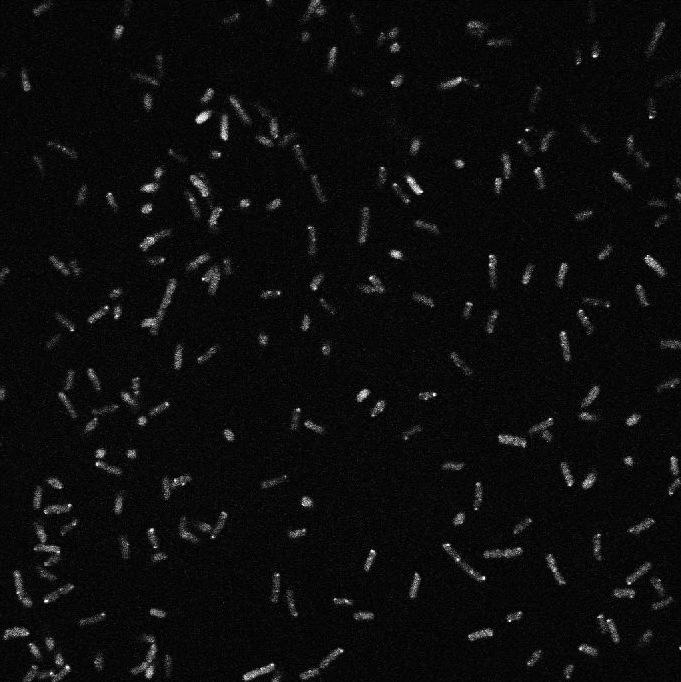
\includegraphics[scale=0.25]{\docroot matmeth/figs/slide1}
	\label{fig:imageprocessing:raw}
}
\subfigure[Edge detection]{
	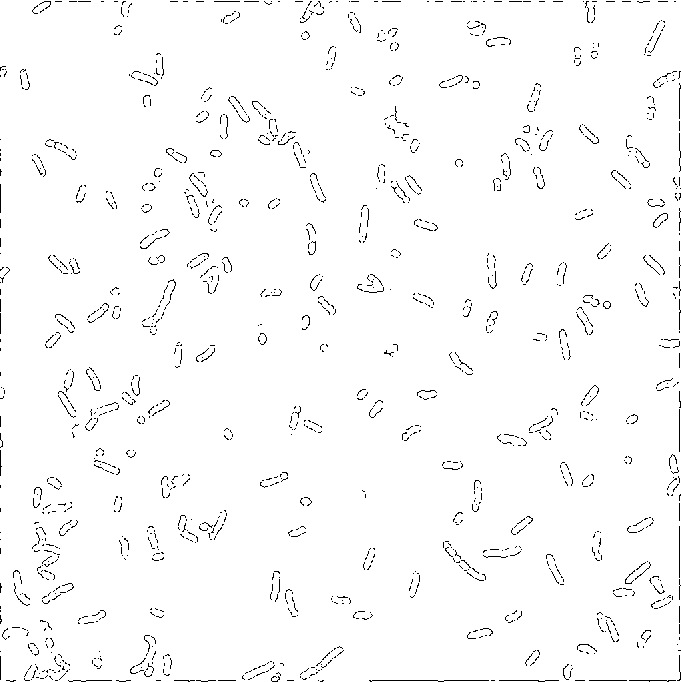
\includegraphics[scale=0.25]{\docroot matmeth/figs/slide2}
	\label{fig:imageprocessing:edges}
}\\
\subfigure[Detected Cells]{
	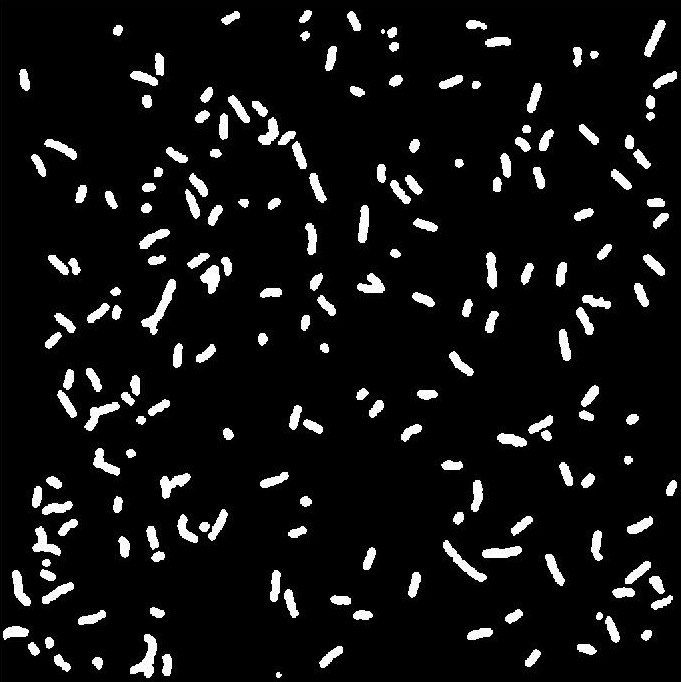
\includegraphics[scale=0.25]{\docroot matmeth/figs/slide3}
	\label{fig:imageprocessing:cells}
}
\subfigure[Accepted Cells]{
	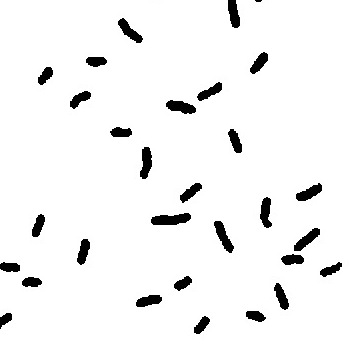
\includegraphics[scale=0.25]{\docroot matmeth/figs/slide4}
	\label{fig:imageprocessing:accepted}
}
\caption{To generate the mask of cells, the script first performs edge detection using the Canny method\cite{canny} (figure~\ref{fig:imageprocessing:edges}). This is particularly effective for detecting edges in noisy images. The lines are then thickened and the gaps closed to give the outline of cells. These are filled in, and then the image is opened with a disk shaped element to remove any small blobs or bridges. This intermediate image is now \texttt{all\_cells} (figure~\ref{fig:imageprocessing:cells}). Subsequently, each constraint on cell shape or size is applied individually to determine which cells to reject (figure~\ref{fig:imageprocessing:accepted}).}
\label{fig:imageprocessing:celldetection}
\end{center}
\end{figure}




\paragraph{cluster\_finder.m}\ \\
\texttt{[ cluster\_fraction, com\_pass, com\_fail ] = cluster\_finder( image, cell\_mask, all\_cells, pixel\_size, threshold, search\_radius, min\_cluster\_size, max\_cluster\_size ) }
\\\\
This function takes as its inputs the image of the cells, and the first two cell masks as described in the previous function. Along with these it takes the following parameters:
\\\\
\begin{tabular}{rl}
Pixel Size		&	Length of pixel in microns\\
Threshold		&	Minimum intensity for peak of cluster, relative to mean cell intensity\\
Search Radius 	&	Radius in which to search for cluster in microns\\
Minimum cluster size	&	Smallest radius of cluster in microns\\
Maximum cluster size	&	Maximum radius of cluster in microns
\end{tabular}
\\\\
As its output it provides a vector containing, for each cluster, the fraction of protein in the whole cell that was found in the cluster. It also contains two vectors containing the centres of mass of each identified cluster and each cluster that failed to meet the given constraints.

Before searching for clusters, the script subtracts low frequency background noise using a rolling ball average. The script then loops through each cell, trying to locate each cluster, through the method shown in figure~\ref{fig:imageprocessing:clusterdetection}.

\begin{figure}[h!]
\begin{center}
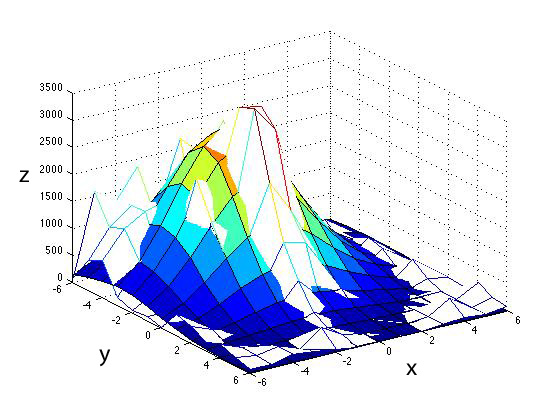
\includegraphics[scale=0.5]{\docroot matmeth/figs/slide5}
\caption{Because the clusters are on the order of the resolution of the microscope (\SI{200}{\nano\meter}), they can be approximated as a 2D Gaussian. To do this, the script finds the brightest pixel not yet masked in the cell, and attempts to fit a 2D Gaussian curve using non-linear optimisation, and masks off the surrounding area from further search. The 2D Gaussian curve is then used to approximate the proportion of fluorescent proteins detected within the cluster compared to the entire cell. This continues until no pixels brighter than the threshold can be found, and the script moves on to the next cell.}
\label{fig:imageprocessing:clusterdetection}
\end{center}
\end{figure}



\subsubsection{Image Alignment}

The OptoSplit II provided by Cairn Research allows for viewing two channels on the same sensor simultaneously. However, as the two images are adjacent in the same file, this requires you to create an alignment so that the two images may be accurately overlaid. This can be automated using some fairly simple mathematical methods.

The two images are extracted with a \(\simeq10\%\) safety border. A mean is taken of each image in each of the x and y axes. A least-squares fitted straight line mean is subtracted from each to negate the effect of any gradient across the image. Each pair of means is then aligned by gradient descent of the root mean square of the difference between them.

This provides the six data points required to align all future images taken until the OptoSplit II is adjusted again - the size of the image, and both of the locations.

Again, all scripts are available online, see section~\ref{sec:scripts:anisotropy}.

\subsection{Microfluidics}

In order to obtain live imaging of the direct response to chemotactic proteins\myfootnote{As opposed to responses induced by blue light}, we must be able to replace the media in which the cells are contained with media of differing concentrations of attractant or repellent. Inspired by Howard Berg and Steven Block's work\cite{berg84} we set out to create a microfluidics flow cell that would allow for precise exchange of media. Aladdin pumps from WPI-Europe were used due to their relatively well documented scripting capabilities and economy - precision was not as pressing concern as normally found in microfluidic applications. Two different microfluidic channels were required.

The first is a simple Y shaped splitter with only one syringe active at any time. One syringe would be filled with a plain media, and the other with media with attractant/repellent at a set concentration. This allows for rapid switching on and off of the attractant/repellent.

The second is a more complex splitter to allow for thorough mixing of the two inputs. This takes the form of a zig-zag style channel between the two inputs and the chamber containing bacteria. Again, one syringe would be filled with a plain media, and the other with media with attractant/repellent at a set concentration. By varying the relative rates of the two pumps but keeping the total constant the concentration of attractant/repellent can be varied between zero and the aforementioned concentration. The drawback of this system is firstly the lag between changing pump speeds and observing a change in concentration in the bacterial chamber, and secondly the smoothing of a step change in concentration due to forward and backward diffusion of the attractant/repellent.

Flow cells were constructed from PDMS before being bonded to \#1.5 glass coverslips. Poly-l-lysine was used to coat the inside of the bacterial chamber by infusing a small amount, withdrawing and then flushing with water. Bacterial cells were then applied by infusing a prepared sample, then flushing with PBS.

\subsection{MicroManager}

In order to give maximum flexibility, the microscope and all related equipment were controlled using MicroManager\cite{micromanager}, an open source software package for control of microscope and associated devices. A beanshell driver was written for the syringe pumps to allow easy integration into experimental workflow, along with several scripts to run experiments. Latest versions of these may be found online, see section~\ref{sec:scripts:micromanager}.

\end{document}
